% This is a sample document using the University of Minnesota, Morris, Computer Science
% Senior Seminar modification of the ACM sig-alternate style. Much of this content is taken
% directly from the ACM sample document illustrating the use of the sig-alternate class. Certain
% parts that we never use have been removed to simplify the example, and a few additional
% components have been added.

% See https://github.com/UMM-CSci/Senior_seminar_templates for more info and to make
% suggestions and corrections.

\documentclass{sig-alternate}
\usepackage{color}
\usepackage[colorinlistoftodos]{todonotes}
\usepackage{multirow}
\usepackage{graphicx}

%%%%% Uncomment the following line and comment out the previous one
%%%%% to remove all comments
%%%%% NOTE: comments still occupy a line even if invisible;
%%%%% Don't write them as a separate paragraph
%\newcommand{\mycomment}[1]{}

\begin{document}

% --- Author Metadata here ---
%%% REMEMBER TO CHANGE THE SEMESTER AND YEAR AS NEEDED
\conferenceinfo{UMM CSci Senior Seminar Conference, April 2017}{Morris, MN}

\title{Automating Algorithm Design through Genetic Programming Hyper-heuristics}

\numberofauthors{1}

\author{
% The command \alignauthor (no curly braces needed) should
% precede each author name, affiliation/snail-mail address and
% e-mail address. Additionally, tag each line of
% affiliation/address with \affaddr, and tag the
% e-mail address with \email.
\alignauthor
Elsa M. Browning\\
	\affaddr{Division of Science and Mathematics}\\
	\affaddr{University of Minnesota, Morris}\\
	\affaddr{Morris, Minnesota, USA 56267}\\
	\email{brow3924@morris.umn.edu}
}

\maketitle
\begin{abstract}
	Automating algorithm design is a current subject of research in several different fields. One field that has approached it is hyper-heuristic optimization. Hyper-heuristics are search functions which seek to automate the process of selecting, generating, or adapting several simpler heuristics in order to solve computational search problems. This process is usually done with machine learning techniques, but this paper explores using a family of algorithms within Evolutionary Computation. Specifically, a genetic programming hyper-heuristic known as autoconstruction.
\end{abstract}

\keywords{Evolutionary Computation, Genetic Programming, Hyper-heuristics, Autoconstruction}

\section{Introduction}
\label{sec:introduction}
Designing algorithms is difficult and time consuming. Because of this, since at least the 1950s, engineers have been trying to automate algorithm design~\cite{pappa:2014}. When we say `trying to automate algorithm design' this means we have been trying to reduce the amount of work people put in to the design process and have been trying to increase the amount of work the computer puts in. Two major approaches to this problem are meta-learning, in the field of supervised machine learning, and hyper-heuristics, in the field of optimization~\cite{pappa:2014}. We will be focusing on hyper-heuristic optimization in this paper.

Hyper-heuristics are heuristic search methods which seek to automate the process of selecting, generating, or adapting several simpler heuristics in order to solve computational search problems. A \textit{heuristic} is a function that ranks alternatives in a search algorithm at each branching step and uses that information to choose which branch to follow. The goal of a heuristic is to find a solution in a reasonable amount of time that is capable of solving the problem at hand.

When designing hyper-heuristics, engineers can use several different kinds of algorithms to automate the process of selecting, generating or adapting simpler heuristics. When genetic programming~(GP) is used for this process, we refer to these as genetic programming hyper-heuristics. GP is a family of algorithms within Evolutionary Computation~(EC), a subfield of Artificial Intelligence. EC encompasses algorithms that use techniques based on biological evolution to solve problems. GP uses these techniques to specifically evolve programs which then solve problems. There are many variations of GP, and the variant used may affect the success of the genetic programming hyper-heuristic.

Traditionally, the system designer determines how GP solutions evolve \cite{spector:2016}. In a newer technique, called autoconstruction, the methods for evolution are evolving as well. Autoconstruction can be thought of as a more complex genetic programming hyper-heuristic.

In this paragraph, we will discuss the layout of this paper. In Sections~\ref{sec:evocomp},~\ref{sec:GP},~and~\ref{sec:HH} we describe background necessary for understanding the rest of this paper. Next, we describe the history of automating algorithm design with a focus on hyper-heuristics optimization in Section~\ref{sec:history}. Then, in Section~\ref{sec:gpvariants}, we outline an experiment that tests different GP variants used in hyper-heuristics and we go into detail on stack-based GP (a genetic programming variant). Next, we will go over current research being done with stack-based genetic programming in Section~\ref{sec:ac}; we briefly discuss Push, a stack-based programming language, along with a technique for automating algorithm design called autoconstruction. Finally we will go over the results of the recent research and some conclusions in Sections~\ref{sec:results}~and~\ref{sec:conclusion} respectively.

\section{Background}
\label{sec:background}
In this Section, we introduce a lot of terminology used throughout the rest of this paper. We also briefly go over the history of hyper-heuristic development.

\subsection{Evolutionary Computation}
\label{sec:evocomp}
Evolutionary Computation (EC) is a subfield of Artificial Intelligence that uses algorithms based on biological evolution to evolve potential solutions to problems. We will describe the general process of an EC algorithm and define the basic terminology. Note that this is not how all EC algorithms work~--~it depicts the most common process.

These algorithms start with a group, or \textit{population}, of randomly generated potential solutions to a problem or set of problems. We measure the quality of these potential solutions, or \textit{individuals}, using a fitness function. This process is referred to as a \textit{fitness test}. Next a selection method is used to pick individuals for reproduction, based on the results of the fitness test; this means the more \textit{fit} individuals, or higher quality solutions, are the ones selected for reproduction. We then apply operations like \textit{mutation}, an insertion, deletion, or small change in an individual, and \textit{crossover}, when two or more individuals are combined in some way to create a new individual, on these individuals to build new solutions. When these operations are applied to potential solutions, the original individual would be referred to as the \textit{parent}, and the new individual would be referred to as a \textit{child}. Parents can have more than one child. Depending on the EC algorithms used, entirely new individuals, usually consisting of entirely random code, are introduced into the next population as well. The next population would be referred to as the next \textit{generation} of potential solutions. This process is repeated on this new generation. We continue to repeat this process until the \textit{global optima}, the best solution (or solutions) possible, is found, or until the algorithm hits a stopping point, such as a time limit or a limit on the number of generations. Stopping points vary from system to system and are implemented to make sure the algorithm run time is fast~--~an algorithm that can find the global optima, but takes a year to do it, is not a very good algorithm.

EC has many applications in medicine, engineering, and chemistry to name a few. Part of the field's success comes from its versatility~--~some examples of EC algorithms include genetic algorithms, which are commonly used to generate high-quality solutions to search and optimization problems, ant colony optimization, which can be reduced to finding good paths through graphs, and artificial immune systems, which are computationally intelligent, rule based machine learning systems. In this paper, we will be focusing on a family of algorithms within EC called genetic programing.

\subsection{Genetic Programming}
\label{sec:GP}
Most EC algorithms produce solutions in the form of a single answer or set of answers to a problem. In genetic programming (GP), our solutions are in the form of programs~--~more specifically, they are usually in the form of trees of operations and values which represent programs. These programs then solve a problem (or set of problems), adding a level of abstraction to the problem solving process. This also automates a large part of the algorithm design process by allowing an algorithm to evolve rather than designing and revising the algorithm by hand.

GP works by encoding programs into a set of genes. These \textit{genes} can be thought of as a reorganization of a program for the evolution process. We then modifying those genes with a genetic algorithm to evolve a program which will perform well on a predefined task. The methods used to encode the programs into \textit{artificial chromosomes}, a structure that holds the genes, and to evaluate the fitness of a program remain active research areas. There are several different GP representations and variations, but we go into more detail on this in Section~\ref{sec:gpvariants}.

\subsection{Hyper-heuristics}
\label{sec:HH}
Before we can understand hyper-heuristics, we must define heuristic. A \textit{heuristic} is a function that ranks alternatives in a search algorithm at each branching step and uses that information to choose which branch to follow. It uses \textit{domain knowledge}, or knowledge about the problem, to find solutions more quickly. If we look at the knapsack problem\footnote{the knapsack problem: given a set of items, each with a weight and value, determine the number of items to include in a collection so that the total weight is less than or equal to a given limit and the total value is as large as possible.}, a heuristic might be, given list X, ``take the highest value item out of list X and put it into the knapsack. If the knapsack will be overweight, take the next highest valued item instead, etc. Repeat this process until the knapsack is full." The heuristic uses the total weight a knapsack can hold and value of the items to find a solution to this problem.

\textit{Hyper-heuristics} are heuristic search methods which seek to automate the process of selecting, generating, or adapting several simpler heuristics in order to solve computational search problems. These work indirectly on the solution space and work directly on the space of heuristics to solve problems~\cite{tauritz:tutorial}. Hyper-heuristics also work on the space of \textit{metaheuristics}, which are more generalized heuristics that do not need domain knowledge to solve the problem; in other words, metaheuristics are not problem specific~\cite{tauritz:tutorial}. Hyper-heuristic design has two major components; the first is to create a set of algorithmic primitives appropriate for tackling a specific problem class and the second is searching that algorithmic primitive space~\cite{harris:2015}. \textit{Algorithmic primitives} is a vague term because it is problem dependent; for example, when playing chess, your \textit{primitives} would the set of possible moves for each of your chess pieces for an individual board state. The \textit{algorithm} would then find ways to use these primitives to determine the best move to make in that board state. Genetic programming is used for the second part in genetic programming hyper-heuristic design.

\subsection{History of Hyper-heuristics}
\label{sec:history}
%Automating algorithm design has been investigated by several different areas for at least 60 years. In the 1950s, the term ``machine learning" was defined as ``computers programming themselves"~\cite{pappa:2014}. This definition has changed over time to focus more on the learning aspect, but machine learning is still used to tackle the problem of automating the design of algorithms. While it plays an important role in the history of attempting to automate algorithm design, machine learning is out of the scope of this paper so it will not be discussed further.%

Focusing on the automation of heuristic development, we can trace the beginnings of hyper-heuristics to the 1960s (however, the term `hyper-heuristic' was not coined until 2000). Early approaches to developing hyper-heuristics focused on automatically setting the parameters of evolutionary algorithms. A \textit{parameter} used to be thought of as things like mutation and crossover rates, however the definition has expanded to include evolutionary algorithm components like selection mechanisms, and mutation and crossover operators. Many researchers still question which parameters to tune when designing hyper-heuristic systems. Traditionally, parameters are tuned before the evolution starts and controlled during the evolution. There are, however, exceptions. The idea of \textit{self-adaption}, where an algorithm is able to evolve parameters while solving a given problem (see Section~\ref{sec:ac}), emerged later.~\cite{pappa:2014}

Today there are two major types of hyper-heuristics: \textit{heuri\- stic selection} and \textit{heuristic generation}; the first focuses on selecting the best algorithm from a set of existing heuristics while the latter focuses on generating a new heuristic from the components of existing heuristics~\cite{pappa:2014}. The \textit{components} can be anything from the code of a heuristic function; this means it could be \textit{instructions}, for example adding two numbers together or determining if two strings are identical, or \textit{literals}, such as strings, integers, booleans, etc. We will be focusing on an example of heuristic generation in Section~\ref{sec:autodog}.

\section{Genetic Programming Variants}
\label{sec:gpvariants}
In genetic programming hyper-heuristics, genetic programming~(GP) can be used for heuristic and program evolution. However, there are many different \textit{genetic programming variants}, or variations on the representation and setup of GP algorithms. Does it matter which variants engineers use in their hyper-heuristics? Harris et al.~\cite{harris:2015} addresses this question; they performed an experiment with five different GP variants to see if the variant chosen affects the success of a hyper-heuristic. The variants tested were Tree-based GP, Linear GP, Cartesian GP, Grammatical Evolution, and Stack-based GP (see Harris et al.~\cite{harris:2015} for details about each of these variants). All of the listed variants were tested on the Boolean Satisfiability Problem~(SAT)\footnote{Harris et al. actually use a subproblem of SAT called 3-SAT. More information about the problem can be found in~\cite{harris:2015}}; the SAT problem is known for its complexity and NP-compl\-eteness\footnote{This is why Harris et al. chose SAT. To be \textit{NP-complete} means there is no known polynomial solution, and it is believed that one does not exist.}. SAT is also useful because many other difficult problems can be reduced to it. 

We will discuss the details of stack-based GP due to its relevance in Section~\ref{sec:ac} and then go over the experiment and results of Harris et al. in Section~\ref{sec:gpresults}.

\subsection{Stack-based Genetic Programming}
\label{sec:sgp}
\begin{table}
	\centering
	\begin{tabular}{|r|c|c|c|c|c|c|c|}
		\hline
		Input & 2 & 1 & \texttt{add} & 2 & \texttt{mult} \\
		\hline
		\multirow{3}{*}{Stack} & & & & &\\
		&   & 1 &   & 2 &   \\
		& 2 & 2 & 3 & 3 & 6 \\
		\hline
	\end{tabular}
	\caption{Each column shows an input element and the contents of the Stack after processing that input.}
	\label{tab:stacks}
\end{table}

Stack-based GP~(SGP) uses data-stacks to manage the input and output of operations. To explain data-stacks, it's helpful to look at an example. If we have the program $((2+1)*2)$, we would first put it into \textit{postfix} notation, which is where any arguments or parameters for a command are stated before that command: \texttt{2~1~add~2~mult}. We do this because SGP are represented as linear sequences and postfix notation is a good way to put programs into this format. In the program, \texttt{add} means take two numbers off the top of the stack, add them together, and push the result back onto the stack. And \texttt{mult} means the same thing except multiply instead of add the numbers.

In Table~\ref{tab:stacks}, this program is shown being input into a stack. When the stack encounters \textit{terminals}, such as strings, integers, booleans, etc., they are simply pushed onto the stack. When the stack encounters \textit{primitives}\footnote{This was defined early in the paper under \textit{algorithmic primitives}, but this definition is different because `primitive' means different things depending on the context}, which are things like subtraction, string length, greater than, etc. they are executed by taking elements off of the stack and pushing their results back onto the stack. For instance, if we look at the first part of the program, \texttt{(2~1~add)}, we would push the 2 and 1 (which are terminals) onto the stack and then execute the add (which is a primitive). The add is executed by popping the top integer off of the stack, which would be 1, and popping the second integer off of the stack, which would be 2, and adding them together. We would then push the result, 3, back onto the stack. If, say, our program had started with \texttt{2 add} instead, we would push the 2 onto the stack, and skip the add because there would not be enough arguments to execute it. This means the next part of the program would push 2 onto the stack, and execute the \texttt{mult} leaving 4 in the place of the 6 in the table.

At the end of Table~\ref{tab:stacks}, we can see that 6 is left on the stack. Generally, the top item on the stack at the end of a program is the answer to a problem that the program is trying to solve. This example was very simple and only dealt with integers. What happens when we have multiple \textit{data types}, such as integers, strings, booleans, and more? Some SGP will push and pop all of their data from one stack, regardless of the data type. But other SGP languages have multiple data-stacks, where there is a stack for each data type. This means that there is an execution stack, where the program is evaluated, and separate stacks that the data is pushed onto and popped off of depending on the data type. Section~\ref{sec:push} shows an example of a SGP with multiple stacks.

SGP are useful for hyper-heuristics because of the ability to skip instructions. This means, for example, that if a terminal is deleted from a program during the evolution phase, the program can still execute.

\subsection{Results}
\label{sec:gpresults}
\begin{figure}
	\centering
	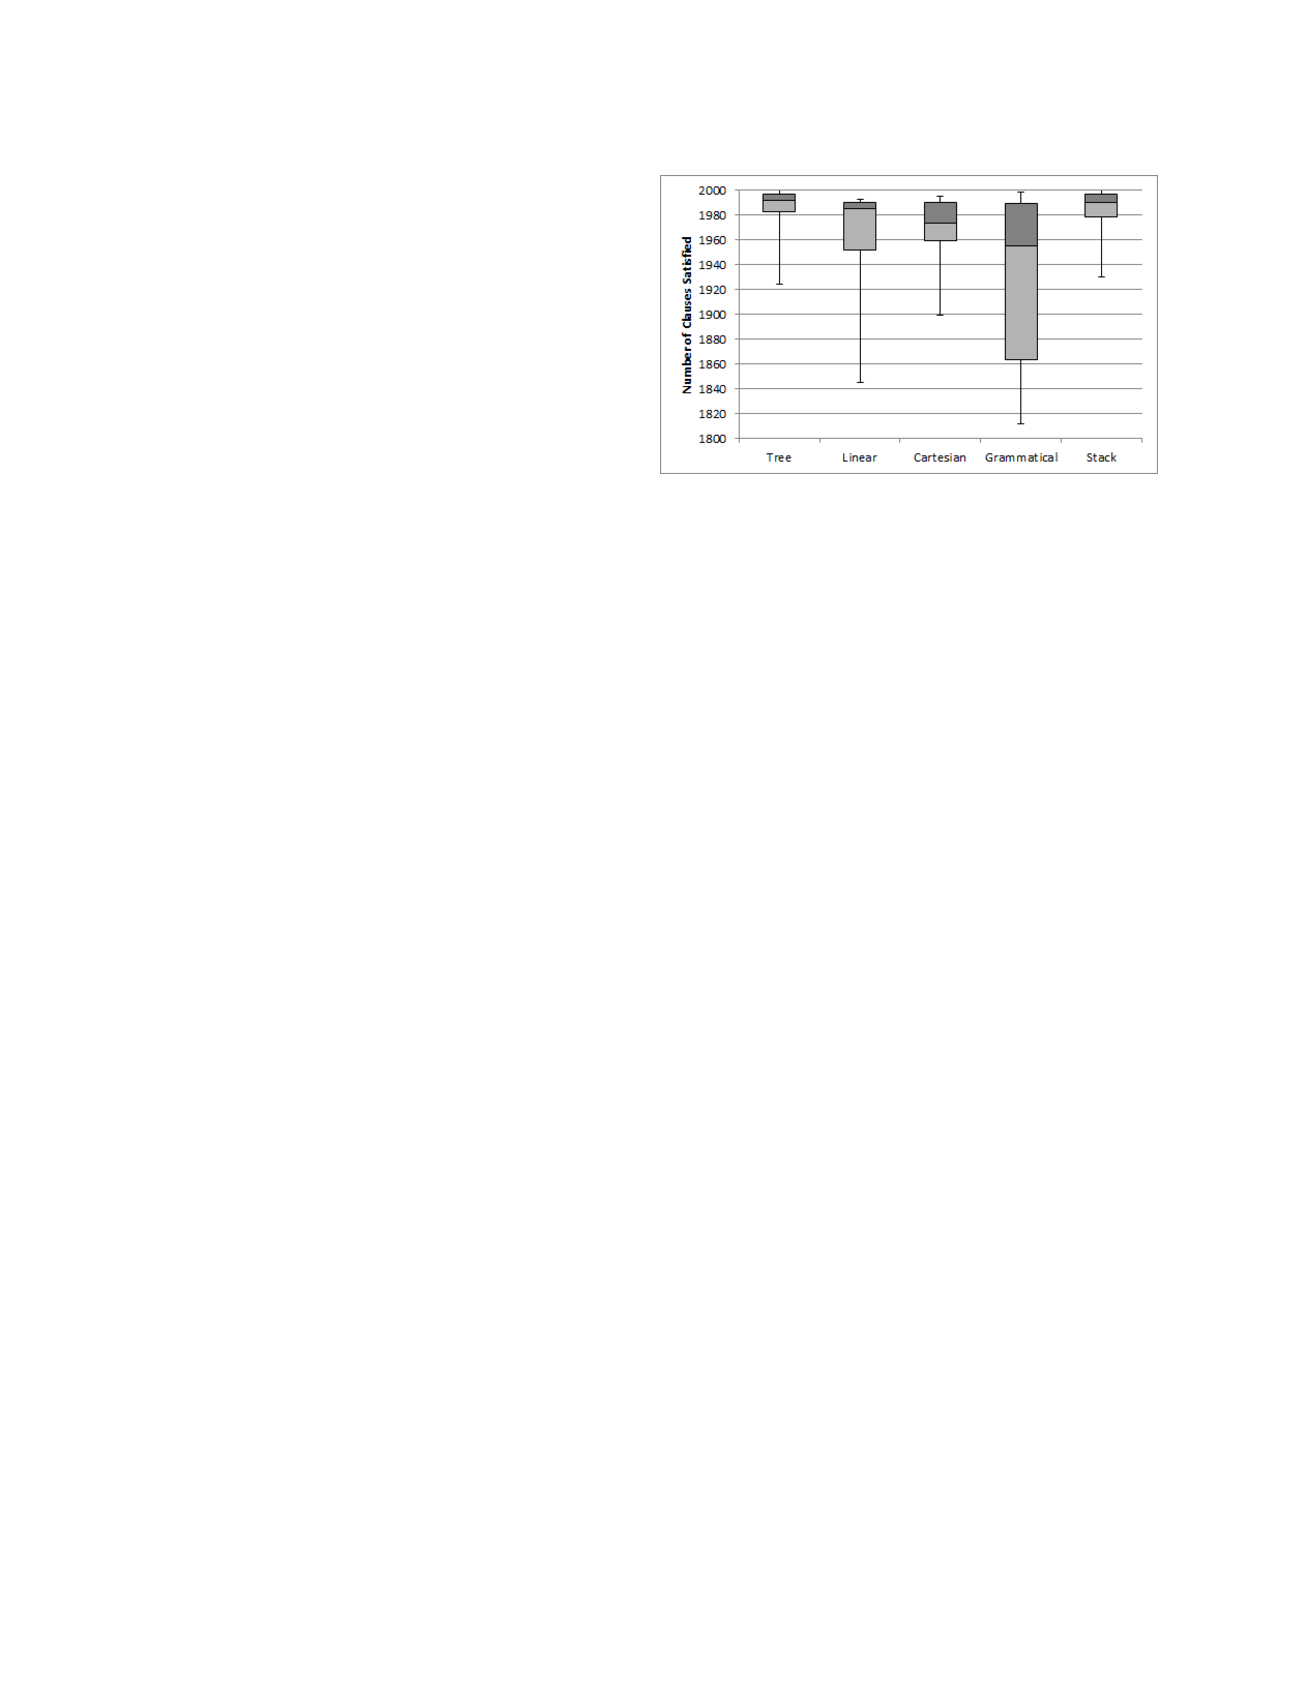
\psfig{file=gpvariant_graph.pdf,width =3.2in}
	\caption{Box plot showing the average number of SAT problem clauses that are satisfied by the best individuals from each run on the test set~\cite{harris:2015}.}
	\label{fig:gpvariants}
\end{figure}

To determine any differences in performance, the five GP variants were implemented in a common framework which facilitated sharing as much code as possible. This implementation causes bias in the results, but this was selected to maintain a common implementation. The alternative, attempting to maximize the performance of each GP variant at the cost of keeping a common implementation for all of the GP variants, would cause similar bias~\cite{harris:2015}.

The GP variants were tested on an instance of the SAT problem. Specifically, the hyper-heuristics (using these GP variants) were evaluated on all 2000 subproblems, or \textit{clauses}, within the instance given to determine how well each hyper-heuristic solves the problem. First each hyper-heuristic (which is the same except for the GP variant used) is run 30 times on a separate set of SAT clauses to `train' the hyper-heuristic. After each run, the best individual program from each hyper-heuristic is tested on the 2000 test clauses 3 separate times. These results are shown in Figure~\ref{fig:gpvariants}.

The results from Harris et al.~\cite{harris:2015} show that the GP variant chosen has a significant impact on the success of the hyper-heuristic. Tree-based GP and stack-based GP performed the best and performed similarly to one another. They solved more clauses of the SAT problem on average than the other GP variants. Linear and Cartesian GP performed similarly to each other, but were not quite as good. Grammatical Evolution performed the worst. This does not mean that tree and stack are inherently better than other GP variants~--~it means that GP variants have different strengths and some are more suited to certain problem spaces than others. More testing is needed to determine how the GP variant used can cause a hyper-heuristics system to excel.

\section{Autoconstruction}
\label{sec:ac}
Autoconstruction is a genetic programming hyper-heur\-istic~(GPHH) that uses genetic programming to evolve programs which have heuristic functions available to them to select the best program possible for a problem. 

In most GPHH, the individual programs are evolving, but everything else is specified by the engineer. This means engineers might set half the population to produce children through a mutation that inserts an \textit{element}, a literal or instruction, every ten elements in a program. And they might set the other half to experience crossover where the first half of the code for the child comes from one individual and the second half comes from another individual. In autoconstruction, engineers don't specify how programs construct their offspring. Instead, the methods of variation are encoded into the programs that are evolving so that, as a program evolves, its variation methods also evolve. An example of this is provided in Section~\ref{sec:autodog}.

Prior work on autoconstruction has explored a variety of system designs, but, until recently, they have only been able to solve simple problems, such as Scrabble Score, Vector Sums, etc (see \cite{helmuth:2015} for details). A new system called Autoconstructive Diversification of Genomes (AutoDoG) has broken this trend by solving a problem that many genetic programming systems have struggled with: Replace Space with Newline~\cite{spector:2016}. And, in recent unpublished work, AutoDoG has solved a problem called String Differences that has not been solved by other GP systems before~\cite{eva:2017}.

In Section~\ref{sec:push}, we introduce Push, the programming language used by AutoDoG, and Plush, the linear genome format (defined in Section~\ref{sec:push}) of Push that AutoDoG uses. In Section~\ref{sec:autodog} we highlight some key features of AutoDoG and in Section~\ref{sec:results} we go over AutoDoG's recent success.

\begin{table}
	\centering
	\begin{tabular}{|r|c|c|c|c|c|c|c|}
		\hline
		:exec & 1 & 2 & `hi' & string\_length & integer\_add \\
		\hline
		\hline
		\multirow{2}{*}{:string} & & & & & \\
		& & & `hi' &  &  \\
		\hline
		\multirow{3}{*}{:integer} & & & & 2 & \\
		& & 2 & 2 & 2 & 4 \\
		& 1 & 1 & 1 & 1 & 1\\
		\hline
	\end{tabular}
	\caption{Each column shows an element on the :exec stack and the contents of the other two stacks after processing that element.}
	\label{tab:push}
\end{table}

\vspace{.3cm}
\subsection{Push and Plush}
\label{sec:push}
Push is a stack-based programming language with a separate stack for each data type. It was developed for program evolution and autoconstruction was one of the driving forces behind the original design~\cite{spector:2016}. Push programs are sequences of instructions, constants, and parentheses with only one syntax requirement: the parentheses must be balanced~\cite{lee:2001}. For example, \texttt{((1 `hello') 2 integer\_add string\_length integer\_gt)} is a simple Push program with its parenthesis balanced.

Instructions are executed by putting them on the \texttt{:exec} stack. For example, assume all stacks are empty and assume a program says \texttt{(1 2 `hi' string\_length integer\_add)}. In Table~\ref{tab:push}, we illustrate the execution of this program (there are more types of data stacks, but we only use two for this example). We push the entire program onto the \texttt{:exec} stack to start. Then we push 1 and 2 onto the \texttt{:integer} stack. Next we push the string `hi' onto the \texttt{:string} stack. We then encounter \texttt{string\_length} on the \texttt{:exec} stack. The \texttt{string\_length} instruction takes a string off the \texttt{:string} stack and returns the string length. To execute this instruction, we pop `hi' off the \texttt{:string} stack and push the string length, in this case 2, onto the \texttt{:integer} stack. Next \texttt{integer\_add} will try to execute: the first two integers on the \texttt{:integer} stack (in this case 2 and 2) are popped off, added together, and the result (in this case 4) is pushed back onto the \texttt{:integer} stack. Since there were enough arguments, the instruction executes.~\cite{lee:tutorial}

If, instead, the program was \texttt{(1 2 string\_length integer\_add)} then \texttt{string\_length} would not execute, but \texttt{integer\_add} still would. What would happen is 1 and 2 would be pushed onto the \texttt{:integer} stack and \texttt{string\_length} would be skipped because there were no strings on the \texttt{:string} stack for the \texttt{string\_length} instruction to use. Then \texttt{integer\_add} would execute as normal with 1 and 2 instead, which would leave us with 3 on the \texttt{:integer} stack in the end instead of 1 and 4.

Plush is a linear genome format for Push~\cite{spector:2016}. This means that Plush is a format of the Push language that allows the programs to be stored in linear genomes. \textit{Linear genomes} are an example of an artificial chromosome (see Section~\ref{sec:GP}). In Section~\ref{sec:autodog}, AutoDoG is actually evolving linear genomes and then translating those genomes back into Push programs~\cite{spector:2016}. This allows for methods of variation in a population to be encoded and evolved more easily. We can just think of genomes as the structure which holds programs for the reproduction process.

\vspace{.3cm}
\subsection{AutoDoG}
\label{sec:autodog}
In this Section, we briefly describe some of the key features of AutoDoG.

When designing AutoDoG, Spector et al.~\cite{spector:2016} wanted to maintain diversity in parent selection. To do this, AutoDoG uses Lexicase Selection. Its name comes from the way it filters the population using a kind of ``lexigraphic ordering" of cases. When tested on a benchmark suite of problems taken from introductory programming textbooks and compared to the results of other current GP parent selection techniques, Lexicase Selection allows for the solution of more problems in fewer generations.

AutoDoG works similarly to PushGP, a reasonably standard genetic programming system, but is run with autoconstruction as the sole genetic operator rather than using human designed operators, like muatation and crossover. In PushGP, the rate of mutation and crossover and other parameters are set by the designers. In AutoDoG, instructions for manipulating genomes are created by the designers, but the rate at which these instructions are used and how they are combined changes through the evolution of programs. For example, \texttt{genome\_uniform\_addition} is an instruction which inserts random instructions into a program with a likelihood taken from the top of the \texttt{:float} stack. The number at the top of the \texttt{float} stack changes as a program executes. So depending on where the \texttt{genome\_uniform\_addition} occurs in the program, the rate of \texttt{genome\_uniform\_addition} may be very different from one program to the next.

In AutoDoG, the reproduction process works as follows:
A program that has performed well on the fitness tests has been selected, using Lexicase Selection, for reproduction. We will call this program Mom. Another program has also performed well and is selected~--~we will call this program Dad. Mom and Dad's genomes are both on the :genome stack. Mom (the program) is run with the purpose of making a child. Part of Mom's code is dedicated to reproduction~--~for example, she may have \texttt{genome\_uniform\_addition} in her code which would take her genome and insert code into it. So Mom uses her reproduction code, which may or may not take pieces of dad's genome, and Mom makes a new genome. Mom pushes this onto the \texttt{:genome} stack. This genome holds the code of her child.

Once this child is constructed, there is the concern of whether or not this child will be passed into the next generation. Spector et al.~\cite{spector:2016} was especially concerned about cloning when designing AutoDoG. \textit{Cloning} is when a parent makes a child that is an exact copy of the parent and this child moves on to the next generation. This is a major concern with evolutionary systems because if a program performs well enough on the fitness tests to move on to the reproduction phase, making a child that is an exact copy allows the child to perform equally well on the fitness tests. Most programs do this if allowed because changing the code is risky; if the change is for the worse, then the program's child will not pass its code on to the next generation. Cloning is bad because it prevents the system from exploring more possible solutions, which makes it difficult to find the global optima. It also significantly slows down the rate of evolution.

Most autoconstruction systems have some form of the ``no cloning rule," and AutoDoG has a form of this as well. AutoDoG's version of this requires offspring to pass a more stringent diversification test in order to enter into the next generation. The child genome, created by Mom earlier, contains the code of a program that we will call Pat; this test begins by having Pat take itself as a mate (the way Mom took Dad as a mate). Pat is run and makes temporary children. If the children differ enough from Pat and from each other, Pat will be inserted into the next population and the children will be discarded. If Pat fails this test, a random genome, meaning a genome with randomly generated code in it, is created and the test is repeated on the random genome. If the random genome fails, a blank genome, with no code in it, is generated and inserted into the next generation (this blank genome does not undergo the diversification test). This test allows for a more diverse set of potential solutions and allows exploration of the problem space.

\vspace{.3cm}
\subsection{Results of AutoDoG}
\label{sec:results}
\begin{figure*}
	\centering
	\begin{minipage}[b]{0.4\textwidth}
		%\psfig{file=dlstandard.pdf,width =3in}
		\includegraphics[width=\textwidth]{dlstandard.pdf}
		\caption{DL-distances between parent and child during a single PushGP run on RSWN~\cite{spector:2016}.}
		\label{fig:standard}
	\end{minipage}
	\hfill
	\begin{minipage}[b]{0.4\textwidth}
		%\psfig{file=dlac.pdf,width =3in}
		\includegraphics[width=\textwidth]{dlac.pdf}
		\caption{DL-distances between parent and child for a single autoconstructive run on RSWN~\cite{spector:2016}.}
		\label{fig:ac}
	\end{minipage}
\end{figure*}

One challenging problem AutoDoG has solved is Replace Space with Newline~(RSWN). This problem is taken from an introductory level textbook and is part of a GP benchmark suite of problems used to evaluate how successful a GP system is. RSWN is a software synthesis problem that takes in a string and prints that string with all spaces replaced by newlines; it also must return the integer count of the non-whitespace characters~\cite{helmuth:2015}. This is complex for GP systems because it involves multiple data types, such as strings and integers, and multiple outputs.

AutoDoG solves the RSWN problem 5--10\% of the time, whereas PushGP solves it about 50\% of the time~\cite{helmuth:2015}. Why do we care about AutoDoG when a relatively standard GP system performs much more reliably? We care because autoconstruction automates more of the algorithm design process than other GP systems, so while it may not perform as well on RSWN, it performs better on the problem of automating algorithm design; AutoDog's success may not seem like much, but the fact that AutoDoG solves the problem at all is actually quite impressive. It is not surprising that AutoDoG performs less reliably because AutoDoG has to learn how to construct offspring as well as learn how to solve problems. In recent unpublished work however, there may be examples of autoconstruction performing `better' than PushGP in a more meaningful sense; autoconstruction has found the solution for String Differences which has never been solved with regular PushGP (or any other GP system)~\cite{eva:2017}.

AutoDoG is unique among autoconstructive systems in that it can solve problems that are challenging for other autoconstructive and GP systems\footnote{These problems are not difficult for people to solve~--~in fact they are fairly easy problems taken from introductory level textbooks. However these problems are difficult for GP systems to solve and serve as a set of benchmarks for GP systems to reach~\cite{helmuth:2015}}. However, as stated by Spector et al.~\cite{spector:2016},
\begin{quotation}
	We do not know which of these [AutoDoG's features], or which combinations of these, may be responsible for the fact that AutoDoG appears to be capable of solving more difficult problems than previous autoconstructive evolution systems.
\end{quotation}
This is because it's hard to separate the pieces; there are a lot of intertwined elements of AutoDoG and Push. Separating them to find exactly which elements contribute to the success without unraveling the entire system is difficult and has not yet been accomplished.

One interesting thing to note about AutoDoG is how it evolves. In standard PushGP, one can see a steady incline in Damerau-Levenshtein distance~(DL-distance) between the genomes of parents and their children in Figure~\ref{fig:standard}. A \textit{Damerau-Levenshtein distance} can be thought of as a measure of change between the genomes of a parent and child over the course of a single generation. In Figure~\ref{fig:standard}, over the 150 or so generations, change occurs at a steady rate and is not very dramatic from one generation to the next~--~the most change that occurs is about 200 differences between a parent and child. This is because engineers set the parameters pertaining to biological evolution before they run the program. The scattered dots near the first generation occurs because the first set of individuals is randomly generated. In AutoDoG, there are big differences between the genomes of some parents and their children as shown in Figure~\ref{fig:ac}. Notice how the y-axis goes up to 2500 DL-distance in the AutoDoG graph compared to only about 800 in the PushGP graph. This is due to the fact that, in AutoDoG, the programs are evolving the parameters pertaining to biological evolution. In the AutoDoG graph, we are essentially seeing evolution evolve.

\vspace{.3cm}
\section{Conclusions and Future Work}
\label{sec:conclusion}
Automating algorithm design is a complex problem that has been investigated for over 60 years. We have recently automated a larger part of algorithm design through the use of genetic programming hyper-heuristics, specifically using a technique called autoconstruction. These techniques are important because the closer we come to systems that can reliably generate algorithms from scratch, the closer we come to drastically changing computer science; we could potentially solve problems people have never solved before, let alone dreamed of solving. At the very least we would not need programmers to write simple algorithms anymore because the computer would do this job using genetic programming hyper-heuristic systems, which would drastically change the programming industry.

However, according to Pappa et al.~\cite{pappa:2014} in 2014, machine learning was ahead of hyper-heuristics optimization on the subject of automating algorithm design and ``can operate over different datasets, from different problem domains, and even with different features." This is not to say that machine learning is better than hyper-heuristic optimization, it simply means they are solving a broader range of problems within a single program. Hyper-heuristics are more focused on optimization, or solving problems quickly, so there is still something to be said for hyper-heuristic optimization. And both fields focus on different problems, so while they are comparable, it does not mean research should be lessened in either field.

It would be interesting to see machine learning techniques combined with hyper-heuristics. Cartesian genetic programming (one of the GP variants in harris et al.~\cite{harris:2015}) has a similar structure to neural networks, a type of machine learning technique. It might be interesting to try and combine the two structures. It would also be useful to find out what search spaces each genetic programming variant excels in~--~Harris et al. mentions further investigation in the end of their paper, so we may see work on this in the near future.

\section*{Acknowledgments}
\label{sec:acknowledgments}
Special thanks to Nic McPhee and Elena Machkasova for their time, feedback, and constructive comments. And thanks to Alex Jarvis and Michael Bukatin, my external reviewers.

\vspace{.3cm}
% The following two commands are all you need in the
% initial runs of your .tex file to
% produce the bibliography for the citations in your paper.
\bibliographystyle{abbrv}
% browning_paper.bib is the name of the BibTex file containing the
% bibliography entries. Note that you *don't* include the .bib ending here.
\bibliography{browning_paper}  
% You must have a proper ".bib" file
%  and remember to run:
% latex bibtex latex latex
% to resolve all references

\end{document}